\documentclass[10pt,xcolor=dvipsnames]{beamer}
\usepackage{beamerthemesplit}
\usetheme{CambridgeUS}  %Warsaw, AnnArbor, Singapore, PaloAlto
%\usetheme{Warsaw}
\setbeamertemplate{footline}[frame number]
%\usefonttheme{structurebold}
%\usefonttheme[onlymath]{serif}
\usefonttheme{serif}
\usepackage{pgf,pgfarrows,pgfnodes,pgfautomata,pgfheaps,pgfshade}
\usepackage{amsmath,amssymb}
%\usepackage[latin1]{inputenc}
\usepackage[english]{babel}
\usepackage{times}
\usepackage{hyperref}
\usepackage{colortbl}
\usepackage{helvet}
\setbeamercovered{dynamic}

\newtheorem{thm}{Theorem}
\newtheorem{lem}{Lemma}
\newtheorem{cor}[thm]{Corollary}

\newcommand{\rtn}{\sqrt{n}}

\title{Innovative Trial Designs in Mobile Health}
\author{{\bf Bibhas Chakraborty}$^{1,2}$\\ \small{ $^1${\bf Duke-NUS Medical School} and {\bf Department of Statistics \& Applied Probability,}\\ {\bf National University of Singapore}\\  $^2${\bf Department of Biostatistics \& Bioinformatics, Duke University}}}
\institute{{\color{blue}bibhas.chakraborty@duke-nus.edu.sg}}
\date{\small{Meeting with BRCCH\\Singapore\\ October 21, 2019}}

%\logo{\includegraphics[height=0.5cm, width=1.5cm]{Duke_NUS_new_logo.png}}



\begin{document}

\begin{frame}%[plain]
\titlepage
\begin{center}
\includegraphics[width=2.5cm, height=0.8cm]{Duke_NUS_new_logo.png}
\hspace*{5cm}
\includegraphics[width=2.5cm, height=1.2cm]{NUS_logo.jpg}%}
\end{center}
\end{frame}



\begin{frame}[plain]
\frametitle{My Career Journey in Brief}
\begin{itemize}
\item 07/2009: PhD in Statistics, University of Michigan, Ann Arbor
\item 08/2009 -- 06/2013: Assistant Professor, Department of Biostatistics, Mailman School of Public Health, Columbia University, New York
\bigskip
\item 06/2013 -- 03/2017: Assistant Professor, Centre for Quantitative Medicine (CQM), Duke-NUS
\item 04/2017 -- Present: Associate Professor, CQM, Duke-NUS 
\item 10/2017 -- Present: Associate Professor, Department of Statistics and Applied Probability, Faculty of Science, NUS
\item 11/2017 -- Present: Adjunct Associate Professor, Department of Biostatistics and Bioinformatics, Duke University, Durham
\item 04/2018 -- Present: Associate Professor, Health Services and Systems Research (HSSR), Duke-NUS
\bigskip
\item {\color{blue}08/2014 -- 06/2018: Director, CQM, Duke-NUS}
\item {\color{blue}08/2017: Launched the new PhD program in Integrated Biostatistics and Bioinformatics (now re-branded as Quantitative Biology and Medicine)} 
\end{itemize}
\end{frame}



\begin{frame} %[plain]
\frametitle{Research Team}
\alert{Current Members}
\bigskip
\begin{itemize}
\item {\color{blue}Raju Maiti:} Research Fellow (Duke-NUS)
\item {\color{blue}Yan Xiaoxi:} PhD student, Biostatistics and Health Data Science (Duke-NUS)
\item {\color{blue}Xie Feng:} PhD student, Health Services and Systems Research (Duke-NUS)
%\item {\color{blue}Li Yun} (Research Assistant)
\item {\color{blue}Nina Deliu:} PhD student, Statistics (University of Rome La Sapienza)
\item {\color{blue}Rupsa Roy:} MSc student, Statistics (NUS)
\item {\color{blue}Feng Ling:} BSc Honours student, Statistics (NUS)
\item {\color{blue}Luo Yixuan (Shirley):} BSc Honours student, Statistics (NUS)
\end{itemize}
\bigskip
\alert{Active Alumni (Research Fellows)}
\begin{itemize}
\item {\color{blue}Palash Ghosh:} Assistant Professor, Indian Institute of Technology (IIT), Guwahati, India
\item {\color{blue}Xu Jing (Kenny):} Data Scientist at Children's Medical Research Institute, University of Sydney, Sydney, Australia 
\item {\color{blue}Sedigheh Mirzaei:} Assistant (Faculty) Member at St Jude Children's Research Hospital, Memphis, USA
\end{itemize}

\end{frame}



\begin{frame}%[plain]
  \frametitle{Outline}
  \tableofcontents[part=1]
\end{frame}


\part<presentation>{Main Talk}


\AtBeginSection[] {
  \begin{frame}<beamer>[plain]
    \frametitle{Outline}
    \tableofcontents[current,currentsubsection]
  \end{frame}
}


%\begin{frame}
%\frametitle{Popularity of mHealth}
%\begin{figure}
%\resizebox{4.5in}{2.5in}{\includegraphics{mhealth.png}}
%\end{figure}
%\end{frame}
%
%
%
%\begin{frame}
%\frametitle{Popularity of TeleHealth }
%\begin{figure}
%\resizebox{4.5in}{2.5in}{\includegraphics{telehealth.png}}
%\end{figure}
%\end{frame}


% \begin{frame}%[plain]
%   \frametitle{Outline}
%   \tableofcontents[part=1]
% \end{frame}
% 
% 
% \part<presentation>{Main Talk}
% 
% 
% 
% \AtBeginSection[] {
%   \begin{frame}<beamer>[plain]
%     \frametitle{Outline}
%     \tableofcontents[current,currentsubsection]
%   \end{frame}
% }

% \AtBeginSubsection[] {
%   \begin{frame}<beamer>[plain]
%     \frametitle{Outline}
%     \tableofcontents[current,currentsubsection]
%   \end{frame}
% }
% 
% \section{Novel Designs in Digital Health}

\section{Non-inferiority Testing in SMARTs for Mobile Health}

\begin{frame}
\frametitle{A Weight Loss Management App}
\begin{center}
\includegraphics[height=6cm, width=10cm]{Home-BG.jpg}\\
\bigskip
Source: {\color{blue}https://smartstudy.northwestern.edu/\#homePage}
\end{center}
\end{frame}



\begin{frame}
\frametitle{The Weight Loss Management App: What's Next?}
\begin{itemize}
\item Not everyone is good with technology (e.g., app); some may need human intervention (e.g., coaching)
\smallskip
\begin{itemize}
\item[--] But coaching is more \alert{costly and burdensome}
\end{itemize}
\bigskip
\item Perhaps a \alert{stepped-care approach} involving the app may be \alert{cost-effective}
\smallskip
\begin{itemize}
\item[--] Start with a low-cost, low-intensity intervention (app) first; and then \alert{step up to a high-cost, high-intensity intervention (e.g., coaching) only for individuals who show early signs of non-response} to low-cost, low-intensity intervention
\end{itemize}
\bigskip
\item It would be interesting to study if a ``stepped-care regime'' is almost as good as (\alert{non-inferior} to) a ``more aggressive or resource-intensive regime'' -- if yes, then the stepped-care regime should be selected 
\bigskip
\item This sort of research question can be investigated using a \alert{Sequential Multiple Assignment Randomized Trial (SMART)} design (\emph{Lavori and Dawson, 2004; Murphy, 2005})
%with \alert{non-inferiority (or equivalence)} testing framework
\end{itemize}
\end{frame}



\begin{frame}%[plain]
\frametitle{Sequential Multiple Assignment Randomized Trial (SMART)}
\begin{itemize}
\item \alert{Multi-stage} trials with a goal to inform the development of {\color{blue}adaptive interventions} (or, {\color{blue}dynamic treatment regimes})
\bigskip
\item  Same subjects participate \alert{throughout} (they are followed through stages of treatment)
\bigskip
\item Each stage corresponds to a treatment decision
\bigskip
\item At each stage the patient is \alert{randomized} to one of the available treatment options
\bigskip
\item Treatment options at randomization may be \alert{restricted} on ethical grounds, depending on intermediate outcome and/or treatment history
\bigskip
\item A trial design that mimics clinical practice!
\end{itemize}
\end{frame}



\begin{frame}
\frametitle{A SMART Weight Loss Management Study}
\begin{center}
{\color{blue}ClinicalTrials.gov ID: NCT02997943} 
\end{center}
\begin{itemize}
\item A 12-month, smartphone app based weight loss management study for overweight/obese individuals at the Northwestern University (\alert{PI: Bonnie Spring})
\end{itemize}
\begin{center}
\includegraphics[height=6cm, width=9cm]{Weight-Loss-SMART.png}
\end{center}
\end{frame}




\begin{frame}[plain]
\frametitle{Non-Inferiority Testing Framework}
\begin{itemize}
\item Consider two embedded regimes: 
\begin{eqnarray*}
{\color{blue}d} &=& (App, App^{\alert{R}}VA^{\alert{NR}}), and \\
{\color{blue}d^*} &=& ((App+Coaching), (App+Coaching)^{\alert{R}} VA^{\alert{NR}})
\end{eqnarray*}
(where VA = Vigorous Augmentation; R = Responder; NR = Non-responder) 
\bigskip
\item Here ${\color{blue}d}$ is a novel stepped-care regime (potentially less costly and burdensome), whereas ${\color{blue}d^*}$ is the active control regime (with established evidence)
\bigskip
\item The non-inferiority hypothesis in a SMART tests that the \alert{average efficacy} of a dynamic regime {\color{blue}$d$} is \alert{not inferior} to that of another regime {\color{blue}$d^*$}, with reference to the non-inferiority margin {\color{blue}$\theta$} (depends on \alert{clinical} judgment)
% \vspace{0.25cm}
% \item The \alert{choice} of {\color{blue}$\theta$} depends on \alert{clinical} judgment
\vspace{0.25cm}
\item We have recently developed an \alert{innovative design solution}: power and sample size formulae, as well as the related data analytic strategies for non-inferiority and equivalence testing in a SMART
% \item In non-inferiority testing\footnote{D'Agostino RB, Massaro JM, Sullivan LM (2003). Non-inferiority trials: design concepts and issues-the encounters of academic consultants in statistics. Statistics in Medicine, 22(2): 169-86}, the goal is to show that the \alert{efficacy} of the experimental regime, when compared to an active control regime, is not \alert{below} the pre-specified \alert{non-inferiority margin}
% \bigskip  
% \item A \alert{non-inferiority margin} is the maximum \alert{clinically acceptable difference} from the active control on average that researchers agree to accept in exchange of the secondary benefits (e.g. cost, burden, side-effects) of the new treatment
\end{itemize}
%\bigskip
{\small
\begin{thebibliography}{1}
\bibitem{ghosh2019}
Ghosh P, Nahum-Shani I, Spring B, and Chakraborty B (2019). Non-inferiority and equivalence tests in sequential, multiple assignment, randomized trials (SMARTs). {\em Psychological Methods}: http://dx.doi.org/10.1037/met0000232.
\end{thebibliography}
}
\end{frame}




\begin{frame}
\frametitle{A Web-based Software (Shiny App) for Non-inferiority Testing in SMARTs}
\begin{center}
{\color{blue}https://osf.io/mqpze/}
%{\color{blue}https://palash.shinyapps.io/ni\_eq\_analysis/}
\includegraphics[height=6cm, width=12cm]{Screen-Shot-2019-07-08}
\end{center}
\end{frame}


%
%
%\frame{\frametitle{The Global Epidemic of Diabetes}
%\begin{figure}
%\resizebox{5in}{2.5in}{\includegraphics{Diabetes.jpg}}
%\end{figure}
%Source: Duke Global Health Institute
%}



%\begin{frame}
%\frametitle{mHealth Interventions for Diabetes Management}
%\begin{itemize}
%\item Good glycaemic control is key to managing diabetes and its many complications
%\bigskip
%\item Treatments for Type 2 Diabetes Mellitus (T2DM) include diet, exercise, oral medications and insulin injections
%\bigskip
%\item Initiation of insulin in insulin-naive patients traditionally involves multiple visits to a physician to adjust insulin dose which can be costly and time-consuming
%\smallskip
%\begin{itemize}
%\item[--] Delay in scheduling can result delay in achieving glycaemic control
%\end{itemize}
%\bigskip
%\item \alert{Self-titration for insulin dose calculation} is also an option but many patients hesitate and express uncertainty
%\end{itemize}
%\end{frame}
%
%
%
%\begin{frame}
%\frametitle{The ``Diabetes Pal'' App}
%\begin{itemize}
%\item A smartphone app, developed in Singapore (Duke-NUS and SGH), with an in-built algorithm to compute daily insulin dosage based on lowest of the previous 3 fasting blood glucose (FBG) readings (patients are required to measure their FBG daily and input into the app)
%\end{itemize}
%\includegraphics[height=5cm, width=12cm]{diabetes_pal.png}
%\end{frame}
%
%
%
%\begin{frame}
%\frametitle{The ``Diabetes Pal'' App}
%The \alert{feasibility} of the app to deliver the insulin titration algorithm in insulin-naive patients has been validated in a pilot RCT ($n=66$):\\
%\bigskip
%{\em Bee YM, et al. (2016). A smartphone application to deliver a treat-to-target insulin titration algorithm in insulin-naive patients with type 2 diabetes: A pilot randomized controlled trial. Diabetes Care, 39(10): e174-e176.}
%\end{frame}






%\begin{frame}
% \frametitle{A SMART Design involving The Diabetes Pal App} 
%\includegraphics[height=6.5cm, width=12cm]{smart_schematic.png} 
%\end{frame}




%\begin{frame}
%\frametitle{General Setup}
%\begin{itemize}
% \item \alert{Objective:} compare two embedded regimens in the SMART with continuous outcome
%\vspace{0.5cm}
%\item Embedded regimens are:
% ${\color{red}d_1} = (A, A^{R}N^{1-R}), {\color{red}d_2} = (A, A^{R}(A+N)^{1-R})$ and ${\color{red}d_3} = (N, N^{R} N^{1-R})$ (control regimen), where {\color{red}$R=1$} denotes responder and {\color{red}$R=0$} denotes non-responder
%\vspace{0.5cm}
%\item Two types of regimen-pairs to consider:
%\vspace{0.25cm}
%\begin{itemize}
%\item[--] Regimen-pairs that start with \alert{different} initial treatments (\alert{distinct-path}): $\{d_1, d_3\}$ and $\{d_2, d_3\}$ 
%\vspace{0.5cm}
%\item[--] Regimen-pairs that start with \alert{same} initial treatment (\alert{shared-path}): $\{d_1, d_2\}$ 
%\end{itemize}
%\vspace{0.5cm}
%\item In this talk, we will focus on the \alert{distinct-path} comparison only
%\end{itemize}
%\end{frame}



%\begin{frame}
%\frametitle{General Setup}
%\begin{itemize}
%\item Data structure: $(T_{1i}, R_i, T_{2i}, Y_i)$ for $i=1,\cdots, n$, where
%\vspace{0.25cm}
%\begin{itemize}
%\item[--] $T_1$ and $T_2$ are the treatment assignment variables at the two stages with $T_1 \in \{A, N\}, T_2 \in \{A, N, (A+N)\}$
%\vspace{0.2cm} 
%\item[--] $R$ is the response indicator ($1/0$)
%\vspace{0.2cm} 
%\item[--] $Y$ is the \alert{continuous} end-of-trial primary outcome (e.g. HbA1c value, or its reduction from baseline), and 
%\vspace{0.2cm}
%\item[--] $n$ is the trial size
%\vspace{0.2cm}
%\end{itemize}
%\item $\tau_{T_1}$: \alert{first-stage} randomization probability in favor of treatment $T_1$
%\vspace{0.25cm}
%\item $\tau_{T_1T_2}$: \alert{second-stage} randomization probability for those who started with first-stage treatment $T_1$, in favor of treatment $T_2$
%\end{itemize}
%\end{frame}






%\begin{frame}
%\frametitle{Estimation of Regimen Mean}
%\begin{itemize}
%\item The regimen mean can be estimated by the IPW estimator (Robins et al., 2000):
%\begin{eqnarray}
%\overline{Y}_{d_1} = \sum_{i=1}^{n} W^{d_1}_iY_{i} \Big/ \sum_{i=1}^{n}W^{d_1}_i \nonumber
%\end{eqnarray}
%
%\item A weighted averaging is essential because of the \alert{structural imbalance} 
%\vspace{0.25cm}
%
%\begin{itemize}
%\item[--] The \alert{non-responders} are \alert{re-randomized} at the second stage, but the responders continue with the same treatment
%\vspace{0.25cm}
%
%\item[--] A \alert{responder} receives the treatment sequence $(A,A)$ with probability $\tau_{A}$
%\vspace{0.25cm}
%
%\item[--] A \alert{non-responder} receives the treatment sequence $(A, N)$ with probability $\tau_{A} \times \tau_{AN}$ 
%\end{itemize}
%\vspace{0.25cm}
%
%\item $W^{d_1}_i = \frac{1}{\tau_{A}}$ for a responder and $W^{d_1}_i = \frac{1}{\tau_{A} \times \tau_{AN}}$ for a non-responder 
%\vspace{0.25cm}
%
%\item For large samples, $\widehat{Var}(\overline{Y}_{d_1}) = \frac{1}{n^2}\sum_{i=1}^{n} (W^{d_1}_i)^2(Y_{i} - \overline{Y}_{d_1})^2$ (Murphy, 2005) 
%\end{itemize}
%\end{frame}




%
%\begin{frame}[plain]
%\frametitle{Non-Inferiority Testing Framework}
%\begin{itemize}
%\item Consider two embedded regimes: 
%\begin{eqnarray*}
%{\color{blue}d} &=& (App, App^{\alert{R}}VA^{\alert{1-R}}), and \\
%{\color{blue}d^*} &=& ((App+Coaching), (App+Coaching)^{\alert{R}} VA^{\alert{1-R}})
%\end{eqnarray*}
%(where VA = Vigorous Augmentation) 
%\bigskip
%\item Here ${\color{blue}d}$ is a novel stepped-care regime (potentially less costly and burdensome), whereas ${\color{blue}d^*}$ is the active control regime (with established evidence)
%\bigskip
%\item In non-inferiority testing\footnote{D'Agostino RB, Massaro JM, Sullivan LM (2003). Non-inferiority trials: design concepts and issues-the encounters of academic consultants in statistics. Statistics in Medicine, 22(2): 169-86}, the goal is to show that the \alert{efficacy} of the experimental regime, when compared to an active control regime, is not \alert{below} the pre-specified \alert{non-inferiority margin}
%\bigskip  
%\item A \alert{non-inferiority margin} is the maximum \alert{clinically acceptable difference} from the active control on average that researchers agree to accept in exchange of the secondary benefits (e.g. cost, burden, side-effects) of the new treatment
%\end{itemize}
%\bigskip
%\end{frame}
%
%
%
%\begin{frame}
%\frametitle{Non-Inferiority Testing in SMARTs}
%\begin{itemize}
%\item For two regimes ${\color{blue}d}$ and ${\color{blue}d^*}$ with corresponding regime means {\color{blue}$\mu_{d}$} and {\color{blue}$\mu_{d^*}$} respectively, the hypothesis for the non-inferiority test is
%\begin{eqnarray}
%{\color{blue}H_0: \mu_{d} \leq \mu_{d^*} - \theta} \mbox{ vs. } {\color{blue}H_1: \mu_{d} > \mu_{d^*} - \theta},
%\nonumber
%\end{eqnarray}
%where {\color{blue}$\theta$} is a pre-specified non-inferiority margin ({\color{blue}$\theta > 0$})
%\vspace{0.25cm}
%\item This hypothesis tests that the \alert{average efficacy} of regime {\color{blue}$d$} is \alert{not inferior} to that of the regime {\color{blue}$d^*$}, with reference to the non-inferiority margin {\color{blue}$\theta$}
%\vspace{0.25cm}
%\item The \alert{choice} of {\color{blue}$\theta$} depends on both \alert{statistical} reasoning and \alert{clinical} judgment
%\vspace{0.25cm}
%\item   The unscaled test statistic is {\color{blue}$\bar Y_{d} - \bar Y_{d^*}$}, with mean {\color{blue}$\mu_{d} - \mu_{d^*}$} and variance {\color{blue}$\nu_{d,d^*}$} (obtained from Murphy's calculations)
%\end{itemize}
%\end{frame}
%
%
%
%\begin{frame}
%\frametitle{Test Statistic and Sample Size Calculation}
%\begin{itemize}
%\item Under {\color{blue}$H_0$}, the \alert{large-sample distribution} of the test statistic
%{\color{blue}
%\begin{eqnarray}
%Z_{d,d^*} = \frac{(\bar Y_{d} - \bar Y_{d^*}) - (\mu_{d} - \mu_{d^*})}{\sqrt{var(\bar Y_{d} - \bar Y_{d^*})}} = \frac{\bar Y_{d} - \bar Y_{d^*} + \theta}{\sqrt{\nu_{d,d^*}}} \rightarrow N(0,1) \nonumber 
%\end{eqnarray}
%}
%\vspace{0.25cm}
%
%\item Reject {\color{blue}$H_0$} at level {\color{blue}$\alpha$} and \alert{conclude non-inferiority} if {\color{blue}$Z_{d,d^*} > z_{\alpha}$} (one-sided)
%\bigskip
%
%\item Deriving sample size formula requires large sample approximations and some assumptions
%\bigskip
%
%\item Given a postulated effect size {\color{blue}$\delta = \mu_{d} -\mu_{d^*}$}, the required {\color{blue}$n$} depends on the \alert{difference} between {\color{blue}$\theta$} and {\color{blue}$\delta$}, rather than their \alert{individual values}
%
%\end{itemize}
%\end{frame}
%
%
%
%
%\begin{frame}[plain]
%\frametitle{Equivalence Testing in SMARTs}
%\begin{itemize}
%\item For two regimes ${\color{blue}d}$ and ${\color{blue}d^*}$ with corresponding regime means {\color{blue}$\mu_{d}$} and {\color{blue}$\mu_{d^*}$} respectively, the hypothesis for the equivalence test is
%\begin{eqnarray*}
%{\color{blue}H_0 : \mu_{d} \le \mu_{d^*} - \theta} \mbox{ or } {\color{blue}\mu_{d} \ge \mu_{d^*} + \theta} \mbox{ vs. } 
% {\color{blue}H_1 : \mu_{d^*} - \theta < \mu_{d} > \mu_{d^*} + \theta},
%\end{eqnarray*}
%where {\color{blue}$\theta$} is a pre-specified equivalence margin ({\color{blue}$\theta > 0$})
%\vspace{0.25cm}
%\item Equivalence test actually involves two one-sided tests (Schuirmann, 1987), one of them being the non-inferiority test 
%\bigskip
%\bigskip
%\item Power and sample size formulae for both non-inferiority and equivalence testing in a SMART, as well as the related data analytic strategies have been developed recently
%\end{itemize}
%
%{\small
%\begin{thebibliography}{1}
%\bibitem{ghosh2019}
%Ghosh P, Nahum-Shani I, Spring B, and Chakraborty B (2019). Non-inferiority and equivalence tests in sequential, multiple assignment, randomized trials (SMARTs). {\em Psychological Methods, in press}.
%\end{thebibliography}
%}
%\end{frame}
%
%
%
%\begin{frame}
%\frametitle{A Shiny App for Non-inferiority \& Equivalence Testing in SMARTs}
%\begin{center}
%{\color{blue}https://osf.io/mqpze/}
%%{\color{blue}https://palash.shinyapps.io/ni\_eq\_analysis/}
%\includegraphics[height=6cm, width=12cm]{Screen-Shot-2019-07-08}
%\end{center}
%\end{frame}



\section{Micro-Randomized Trials in Mobile Health}

\begin{frame}
\frametitle{DIAMANTE App}
\begin{center}
\underline{DIA}betes and \underline{M}ental Health \underline{A}daptive \underline{N}otification \underline{T}racking and \underline{E}valuation
\begin{figure}
\resizebox{4in}{2.5in}{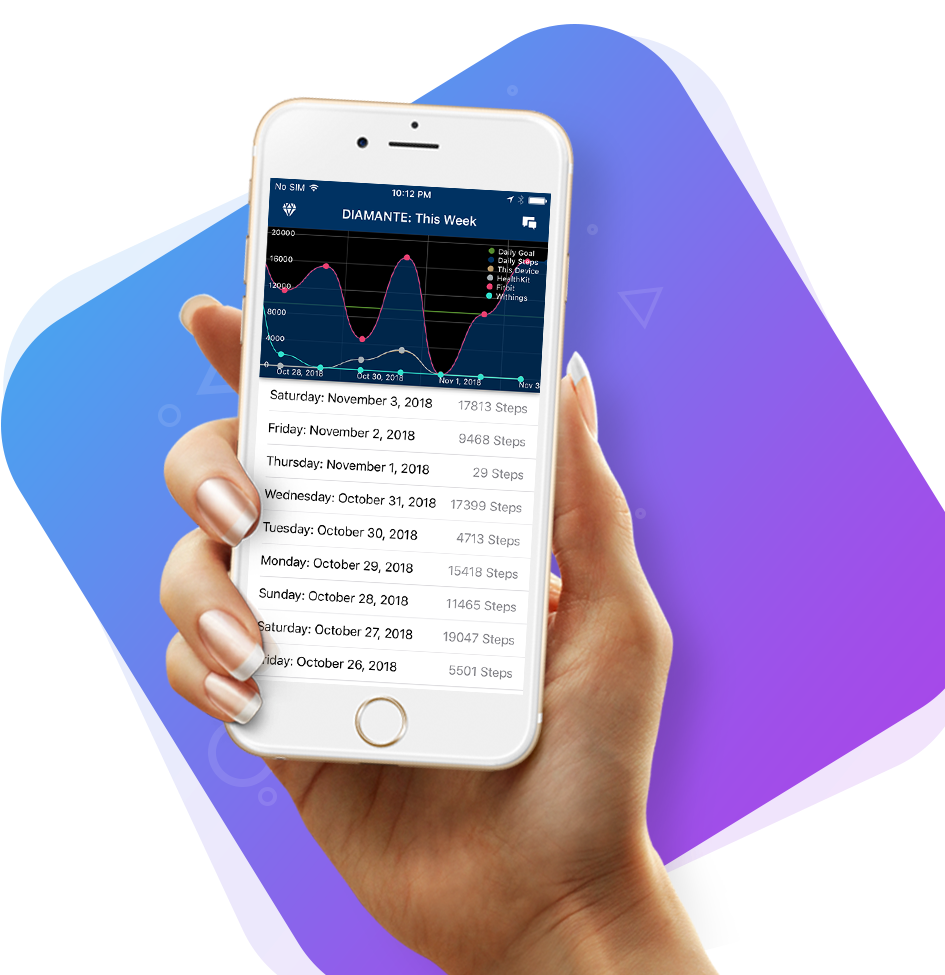
\includegraphics{DIAMANTE_pic.png}}
\end{figure}
Source: {\color{blue}https://diamante.healthysms.org/}
\end{center}
\end{frame}



\begin{frame}
\frametitle{DIAMANTE Study (Trial \#: NCT 03490253)}
%{\small {\em Improving Diabetes and Depression Self-management Via Adaptive Mobile Messaging}}
%\bigskip
Key Collaborators:\\ 
{\color{blue}Adrian Aguilera} and {\color{blue}Caroline Figueroa} (UC-Berkeley), {\color{blue}Courtney Lyles} (UC-SF) and {\color{blue}Joseph Jay Williams} (U-Toronto)
\bigskip
\begin{itemize}
\item \alert{Overarching Goal:} To develop, implement and evaluate an \alert{adaptive-learning}, clinic-integrated mobile intervention targeting {\color{blue}physical activity to manage co-morbid diabetes and depression} in low-income, ethnic minority patients served in the San Francisco Health Network
\bigskip
\item Three-arm RCT: 
\begin{enumerate}
\item \alert{adaptive messaging arm} (daily messages learned by \alert{reinforcement learning}), 
\item static messaging arm (daily health management and educational messages), 
\item control arm (weekly messages about mood and steps)
\end{enumerate}
%\item Specific Aims:
%\begin{enumerate}
%\item \alert{Develop} (conduct user testing of) the DIAMANTE platform.
%\item \alert{Evaluate} the effectiveness of adaptive vs. static messaging intervention.
%\item \alert{Evaluate} the effectiveness of nurse phone outreach for non-responsive participants.
%\end{enumerate}
\end{itemize}
\begin{center}
\alert{Focus on the adaptive messaging arm from now on.}
\end{center}
\end{frame}




\begin{frame}[plain]
\frametitle{Developmental Goal of DIAMANTE Study}
\begin{block}{2 different messages every day, 1 minute apart}
\begin{figure}
\resizebox{3in}{2in}{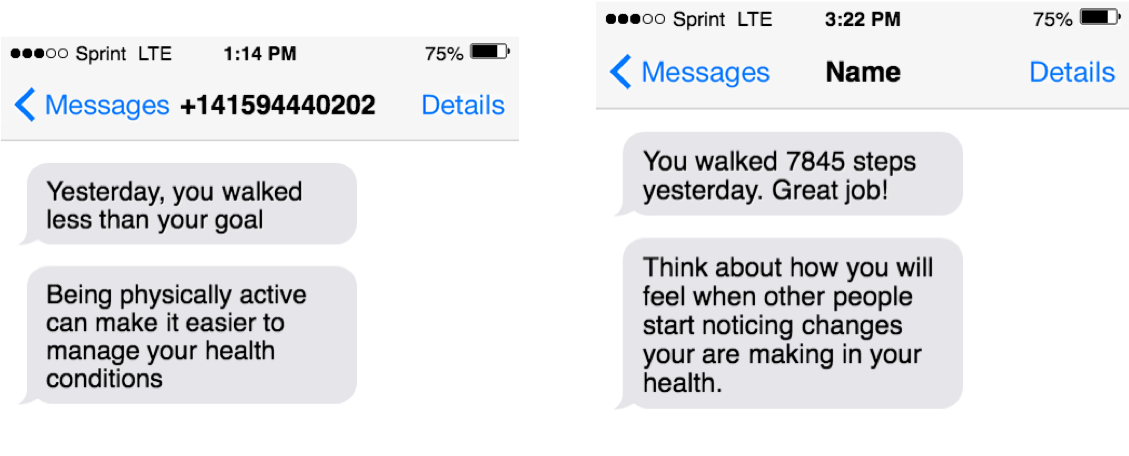
\includegraphics{message-screen.png}}
\end{figure}
\end{block}
\begin{itemize}
\item Learn to send better messages to patients to encourage them to walk more %by continuously learning 
\bigskip
\item Messages are \alert{multi-component interventions, with varying levels} of: (a) Time Window (when to send the message?), (b) Feedback Message, and (c) Motivational Message
\end{itemize}
\end{frame}




\begin{frame}[plain]
\frametitle{Factor 1: Time Window (when to send the message?)}
\begin{figure}
\resizebox{2in}{1.5in}{
\includegraphics{clock.png}}
\end{figure}
\begin{itemize}
\item Level 0: {\em 09:00-11:30}
\item Level 1: {\em 11:30-14:00}
\item Level 2: {\em 14:00-16:30}
\item Level 3: {\em 16:30-19:00}
\end{itemize}
\bigskip
%Feedback message and Motivational message are sent only one minute apart within the chosen window.
\end{frame}




\begin{frame}[plain]
\frametitle{Factor 2: Feedback Message}
\begin{center}
\begin{tabular}{c|l|l}
\hline
Level & Description & Examples \\
\hline
0 & None & -- \\
& & \\
1 & Reaching goal & {\em ``Yesterday, you did not reach}  \\
& & {\em your goal.''} \\
& & \\
2 & Steps walked yesterday & {\em ``Yesterday, you walked 3824}  \\
& & {\em steps.''} \\
& & \\
3 & Walked more/less yesterday & {\em ``Yesterday, you walked more} \\
& than day before & {\em than day before.''} \\
& & \\
4 & Steps walked yesterday,  &  {\em ``You walked 8000 steps yesterday.}  \\
& + a motivational message &  {\em Great job!''} \\
\hline
\end{tabular}
\end{center}

%\begin{itemize}
%\item Level 1: Whether a participant has or has not reached their step goal
%\smallskip
%\item Level 2: The number of steps walked yesterday
%\smallskip
%\item Level 3: The number of steps walked yesterday, PLUS a motivational message
%\smallskip
%\item Level 4: Whether a participant walked more/less today than yesterday
%\smallskip
%\item Level 5: None
%\end{itemize}

% \bigskip
% Within each level, there are multiple possible messages. When a level is selected by the algorithm, one of the possible message will be chosen randomly. %Thus, the participant will receive between 0 to 2 messages per day.
\end{frame}



\begin{frame}
\frametitle{Factor 3: Motivational Message}
\begin{center}
\begin{tabular}{c|l|l}
\hline
Level & Description & Examples \\
\hline
0 & None & -- \\ 
& & \\
1 & Benefit & {\em ``Doing more physical activity can help reduce feelings}  \\
& &  {\em of fatigue.''} \\ 
& & \\
2 & Self-efficacy & {\em ``You have made changes to improve your health before,}  \\
& &  {\em you can do it again.''} \\ 
& & \\
3 & Opportunity & {\em ``It there a local park you have been waiting to visit?}  \\
&  & {\em Use it as an opportunity to get out of the house} \\
&  & {\em and do more steps!''} \\
\hline
\end{tabular}
\end{center}

%\begin{itemize}
%\item Level 1: Benefit message that describes the physical and psychological benefits of engaging in walking and exercise
%\smallskip
%\item Level 2: Self-Efficacy message that is meant to increase self-confidence and the belief that one is capable of walking even in the face of challenges
%\smallskip
%\item Level 3: Opportunity message that identifies physical and social environment cues that make it more likely for someone to engage in walking and exercise 
%\smallskip
%\item Level 4: None
%\end{itemize}
% \bigskip
% Within each level, there are multiple possible messages. When a level is selected by the algorithm, one of the possible message will be chosen randomly. %Thus, the participant will receive between 0 to 2 messages per day.
\end{frame}




%\begin{frame}
%\frametitle{Contextual Variables in DIAMANTE}
%\begin{itemize}
%\item Gender 
%\item Age 
%\item Steps from yesterday
%\item Steps from last 7 days
%\item \% of steps goal achieved yesterday
%\item Progress achieved daily in week thus far (Since Sunday)
%\item For each message category, number of days since message from that category was sent
%\item Weather
%\item GPS location 
%\end{itemize}
%% Here is more details and notes (but in a summarized format) about the project that you can take a look at:
%% https://docs.google.com/document/d/1gvgtKSTKi37NZt5RVxMO_pd3x9no926zmOxjcpDFyl4/edit 
%\end{frame}



\begin{frame}%[plain]
\frametitle{Design Considerations in DIAMANTE Development}
\begin{itemize}
\item \alert{Factorial designs} embedded within the \alert{Multi-phase Optimization Strategy (MOST)} framework are the gold standard when collecting data to build multi-component behavioral interventions ({\em Collins et al., 2005; Nair et al., 2008; Chakraborty et al., 2009})
\bigskip
\item {\color{blue}Micro-randomized trials (MRTs)} ({\em Klasnja et al., 2015}) are cutting-edge trial designs suitable to take care of the time-varying, sequential nature of the interventions 
\smallskip
\begin{itemize}
\item[--] These are sequential, full-factorial designs (as in \alert{MOST})
\item[--] At each decision stage, randomize between possible actions (as in \alert{SMART})  
\item[--] Each person may be randomized at many, many stages (lot more than in \alert{SMART}) 
\end{itemize}
\bigskip
\item Actions are often intended to have a \alert{proximal effect} (unlike \alert{SMART})
\smallskip
\begin{itemize}
\item[--] Randomization is the gold standard in providing data to assess a causal effect
\end{itemize}
\bigskip
\item Continuous outcome: step count in next 24 hours
% from yesterday and day before (= yesterday's steps - day before yesterday's steps).
\bigskip
\item Generalized Estimating Equations (GEE)-type analysis
\end{itemize}
\end{frame}



%\begin{frame}%[plain]
%\frametitle{Why MRTs?}
%\begin{itemize}
%\item Actions are often intended to have a proximal effect
%\smallskip
%\begin{itemize}
%\item[--] Randomization is the gold standard in providing data to assess a causal effect
%\end{itemize}
%\bigskip
%\item Sequential randomization will enhance quality of many interesting subsequent data analyses
%\end{itemize}
%\end{frame}




% \begin{frame}%[plain]
% \frametitle{Towards Designing an MRT for DIAMANTE}
% \begin{itemize}
% \item Key distinguishing features from previous MRTs (e.g. {\em HeartSteps}): 
% \bigskip
% \begin{itemize}
% \item[--] \alert{Availability} is not explicitly considered as a design input (i.e., people are assumed to be available) {\color{blue}[Simplicity]}
% \bigskip
% \item[--] Factors with \alert{more than 2 levels} {\color{blue}[Complexity]}
% \bigskip
% \item[--] Allowance for \alert{adding newer messages} (\alert{``crowdsourcing effect''}) after the trial initiation {\color{blue}[Complexity]}
% \end{itemize}
% \end{itemize}
% \end{frame}



\begin{frame}%[plain]
\frametitle{Towards Designing an MRT for DIAMANTE}
\begin{itemize}
\item Key methodological research questions:
\bigskip
\begin{itemize}
\item[--] How to \alert{power MRTs} involving \alert{factors with more than 2 levels?} 
\bigskip
\item[--] Since we are interested in developmental trials, can the standard \alert{power-based} calculations be replaced by \alert{precision-based} calculations? What is the implication? 
\bigskip
\item[--] How to accommodate \alert{adding new intervention options while in the trial (``crowdsourcing effect")} in sample size calculations?
\bigskip
\item[--] How to \alert{learn online} about more effective intervention components while in the trial? (e.g., {\color{blue}Thompson sampling for contextual multi-arm bandit problems})
\end{itemize}
\end{itemize}
\bigskip
\begin{center}
Currently working on the methods, and also helping the DIAMANTE team with implementation (\alert{Kenny, Xiaoxi, and Nina})
\end{center}
\end{frame}


% \begin{frame}
% \frametitle{Data Structure}
% \begin{center}
% It's a bit more than standard longitudinal data!
% \end{center}
% \begin{itemize}
% \item \alert{$T$ stages (or decision points) on a single individual:}
% \bigskip
% \begin{center}
% {\color{blue}$S_1,A_1,Y_2,\ldots,S_t,A_t,Y_{t+1},\ldots,S_T,A_T,Y_{T+1}$}\\
% \end{center}
% where
% \begin{eqnarray*}
% {\color{blue}S_t} &:& \textrm{Context (pre-treatment) at the {\color{blue}$t$}-th stage}\\
% {\color{blue}A_t} &:& \textrm{Action (treatment) at the {\color{blue}$t$}-th stage}\\
% {\color{blue}Y_{t+1}} &:& \textrm{Proximal Outcome (Response, Reward)}\\
% \end{eqnarray*}
% \item {\color{blue}$S_t$} can be high-dimensional
% \smallskip
% \item {\color{blue}$A_t$} is a \alert{vector} for multi-component interventions (as in DIAMANTE)
% \end{itemize}
% \end{frame}



% \begin{frame}
% \frametitle{Proximal Effect}
% \begin{itemize}
% \item \alert{Principle:} Allow the effect of treatment on proximal outcome to vary with time, potentially accommodating {\color{blue}habituation} and {\color{blue}burden}
% \bigskip
% \item Focus on \alert{one factor} (e.g. motivational message) with {\color{blue}$M$} levels (of message)
% \bigskip
% \item Define the proximal effect of level {\color{blue}$m$} at time {\color{blue}$t$} as
% {\color{blue}$$\beta_m(t) = E(Y_{t+1}|A_t=m) - E(Y_{t+1}|A_t=0),\; m=1,\ldots, M$$}
% where {\color{blue}0} is the reference level (``none'' message) 
% \bigskip
% \item By (slightly) changing notation, it is possible to define effects at time-point {\color{blue}$t$} on {\color{blue}$d$}-th day, say {\color{blue}$\beta_m(d,t)$} 
% \end{itemize}
% \end{frame}




% \begin{frame}[plain]
% \frametitle{Hypothesis Testing}
% \begin{itemize}
% \item Calculate the required sample size in order to test the null hypothesis of no treatment effect, e.g.
% {\color{blue}$$H_0: \beta_1(t)=\ldots=\beta_M(t)=0,\; (t=1,\ldots, T)$$}
% \bigskip
% \item Consider an alternative hypothesis of the generic form
% {\color{blue}$$H_1: \beta_1(t)=Z_t^T\beta_1, \text{or}\; \ldots, \text{or}\; \beta_M(t)=Z_t^T\beta_M,\; (t=1,\ldots, T)$$}
% \bigskip
% \item More specifically, the alternative can be a smooth, low-dimensional function
% {\color{blue}$$Z_t^T\beta_m = [1,(t-1),\ldots,(t-1)^p]\beta_m$$} 
% with {\color{blue}$\beta_m=(\beta_{m1},\ldots,\beta_{mp})^T$} (often \alert{$p=2$, or $p=1$, or an in-between effect})
% \bigskip
% \item GEE-type analysis
% \end{itemize}
% \end{frame}
% 
% 
% 
% \begin{frame}%[plain]
% \frametitle{Input Parameters for Sample Size Calculation}
% \begin{itemize}
% \item For traditional power-based calculation:
% \begin{itemize}
% \item $D$ (number of days in the study)
% \item $T$ (number of decision-times per day), \alert{$T=1$ in DIAMANTE}
% \item Effect size 
% \begin{itemize}
% \item[--] Initial standardized effect
% \item[--] Average standardized effect
% \item[--] Day of maximal effect
% \end{itemize}
% \item Desired power (usually 80\%)
% \item Significance level (usually 5\%)
% \end{itemize}
% \bigskip
% \item For precision-based calculation, desired power can be replaced by {\color{blue}desired precision} (margin of error, half-width of CI)  
% \end{itemize}
% \end{frame}
% 
% 
% \begin{frame}
% \frametitle{Sample Size for 80\% Power ($M=4$)}
% \begin{table}
% %\caption{Sample Sizes estimation based on Power when at least one of the proximal message standardized effect satisfies $\delta_m(d, t)=\boldsymbol Z_{dt}^{\top}\boldsymbol \delta_m$, where $\boldsymbol \delta_m=\boldsymbol\beta_m/\sigma$, for $m=1,\ldots,M$. %Note that we have $M=4$. 
% %Initial standardized effect is 0.02.
% %%The significance level is 0.05. %The desired power is 0.80. 
% %%``Duration" is the duration of study ($D$) in days. 
% %%``Availability" is the availability pattern. ``Max" is the day in which the maximal proximal effect is attained. 
% %%``Decision" is the number of decision time points per day ($T$). 
% %%Linear trend for proximal effect and $100\%$ availability at each time point are assumed.
% %%$\bar{\tau}=(1/DT)\sum_{d=1}^D \sum_{t=1}^{D} E(I_{idt})$ is the average of availability.
% %}
% \label{Table: T1}
% \centering
% \begin{tabular}{rrrrrrr}
%   \hline
% %  & \multicolumn{4}{c}{} & \multicolumn{2}{c}{$\bar{\tau}=1$} \\
%  & \multicolumn{2}{c}{} &  \multicolumn{2}{c}{ Sample Size } & \multicolumn{2}{c}{ Monte Carlo Power } \\
%  & \multicolumn{2}{c}{} &  \multicolumn{4}{c}{ Average Proximal standardized Effect }  \\
%  %& \multicolumn{2}{c}{} &  \multicolumn{4}{c}{ Initial standard effect is 0.02 }  \\ 
%  & $D$ & $T$ & 0.20 & 0.10  & 0.20 & 0.10 \\ 
%   \hline
%  & {\color{blue} 84} &   {\color{blue}1} &  {\color{blue}27} &  {\color{blue}78} & {\color{blue}0.78} & {\color{blue}0.78} \\ 
%  &   &   3 &  17 &  32 & 0.79 & 0.77 \\ 
%  & 28 &   1 &  52 & 190 & 0.79 & 0.80 \\ 
%   &   &   3 &  24 &  70 & 0.76 & 0.80 \\ 
%   & 14 &   1 &  94 & 367 & 0.79 & 0.80 \\ 
%   &   &   3 &  38 & 130 & 0.78 & 0.78 \\ 
%  % & 7 &   1 & 173 & 704 & 0.80 & 0.80 \\ 
%  % &   &   3 &  66 & 250 & 0.80 & 0.79 \\ 
%    \hline
%     \hline
% \end{tabular}
% \end{table}
% \end{frame}
% 
% 
% 
% %\begin{frame}%[plain]
% %\frametitle{Input Parameters for Precision-based SS Calculation}
% %
% %\end{frame}
% 
% 
% 
% \begin{frame}
% \frametitle{Sample Size for Desired Precision ($M=4$)}
% \begin{table}
% %\caption{Sample Sizes estimation based on accuracy when at least one of the proximal message standardized effect satisfies $\delta_m(d, t)=\boldsymbol Z_{dt}^{\top}\boldsymbol \delta_m$, where $\boldsymbol \delta_m=\boldsymbol\beta_m/\sigma$, for $m=1,\ldots,M$. Note that we have $m=4$. The significance level is 0.05.
% % ``Duration" is the duration of study ($D$) in days. 
% % %``Availability" is the availability pattern. ``Max" is the day in which the maximal proximal effect is attained. Linear trend for proximal effect is assumed. 
% % ``Decision" is the number of decision time points each day during the study ($T$). 
% % Linear trend for proximal effect and $100\%$ availability at each time point are assumed.
% % %$\bar{\tau}=(1/DT)\sum_{d=1}^D \sum_{t=1}^{D} E(I_{idt})$ is the average of availability. 
% % Margin error of initial standardized effect is 0.02
% %}
% \label{Table: T2}
% \centering
% \begin{tabular}{rrrrrrr}
%   \hline
%   & \multicolumn{2}{c}{} & \multicolumn{2}{c}{ Sample Size } & \multicolumn{2}{c}{ Coverage Probability } \\
%  & \multicolumn{2}{c}{} &  \multicolumn{4}{c}{Precision}  \\
%  & $D$ & $T$ & 0.25 & 0.15  & 0.25 & 0.15\\ 
%   \hline
%   & {\color{blue}84} &   {\color{blue}1} &  {\color{blue}24} &  {\color{blue}44} & {\color{blue}0.97} & {\color{blue}0.96} \\ 
%  &   &   3 &  17 &  23 & 0.98 & 0.97 \\ 
%  & 28 &   1 &  41 &  93 & 0.96 & 0.95 \\ 
%  &   &   3 &  23 &  40 & 0.97 & 0.96 \\ 
%  & 14 &   1 &  68 & 172 & 0.96 & 0.95 \\ 
%  &   &   3 &  32 &  67 & 0.96 & 0.95 \\  
%      \hline
% \end{tabular}
% \end{table}
% It's possible to size even smaller studies, by considering precision instead of power.
% \end{frame}
% 
% 
% 
% 
% %\subsection{Crowdsourcing: Adding Arms}
% 
% \begin{frame}
% \frametitle{Adding Message Levels Mid-way: 80\% Power-based SS}
% Initially, $M=2$, but 2 additional messages are added mid-way during the trial.
% \begin{table}
% %\caption{Sample Sizes and Monte Carlo power estimation based on power when at least one of the proximal message standardized effect satisfies $\delta_m(d, t)=\boldsymbol Z_{dt}^{\top}\boldsymbol \delta_m$, where $\boldsymbol \delta_m=\boldsymbol\beta_m/\sigma$, for $m=1,\ldots,M_0$,$\ldots$,$\sum_{j=0}^{k}M_j$. Note that we have $M_0=\cdots=M_k=2$, $k=1$, where $d_0=1$ and $d_1$ is the half way through ``Duration" is the duration of study ($D$) in days, e.g., if $D=28$ then $d_1=15$. The significance level 0.05. The desired power is 0.80. ``Decision" is the number of decision time points each day during the study ($T$). Linear trend for proximal effect and $100\%$ availability at each time point are assumed.
% %}
% \label{Table: T3}
% \centering
% \begin{tabular}{rrrrrrr}
%   \hline
%    & \multicolumn{2}{c}{} &  \multicolumn{2}{c}{ Sample Size } & \multicolumn{2}{c}{ Monte Carlo Power } \\
%  & \multicolumn{2}{c}{} &  \multicolumn{4}{c}{ Average Proximal standardized Effect }  \\
%  %& \multicolumn{2}{c}{} &  \multicolumn{4}{c}{ Initial standard effect is 0.02 }  \\ 
%  & $D$ & $T$ & 0.20 & 0.10  & 0.20 & 0.10 \\ 
%   \hline
%   & {\color{blue}84} &   {\color{blue}1} &  {\color{blue}28} &  {\color{blue}81} & {\color{blue}0.77} & {\color{blue}0.80} \\ 
%  &   &   3 &  17 &  33 & 0.79 & 0.78 \\ 
% & 28 &   1 &  60 & 222 & 0.79 & 0.79 \\ 
%  &   &   3 &  27 &  81 & 0.77 & 0.80 \\ 
%  & 14 &   1 & 109 & 429 & 0.79 & 0.80 \\ 
%  &   &   3 &  44 & 152 & 0.79 & 0.81 \\ 
% % & 7 &   1 & 199 & 814 & 0.80 & 0.80 \\ 
% % &   &   3 &  76 & 290 & 0.79 & 0.79 \\ 
%     \hline
%     \hline
% \end{tabular}
% \end{table}  
% \alert{Only minimal increase in sample size requirement!}
% \end{frame}
% 
% 
% 
% \begin{frame}
% \frametitle{Adding Message Levels Mid-way: Precision-based SS}
% Initially, $M=2$, but 2 additional messages are added mid-way during the trial.
% \begin{table}
% %\caption{Sample Sizes and Monte Carlo coverage probability estimation based on accuracy when at least one of the proximal message standardized effect satisfies $\delta_m(d, t)=\boldsymbol Z_{dt}^{\top}\boldsymbol \delta_m$, where $\boldsymbol \delta_m=\boldsymbol\beta_m/\sigma$, for $m=1,\ldots,M_0$,$\ldots$,$\sum_{j=0}^{k}M_j$. Note that we have $M_0=\cdots=M_k=2$, $k=1$, where $d_0=1$ and $d_1$ is the half way through ``Duration" is the duration of study ($D$) in days, e.g., if $D=28$ then $d_1=15$.  The significance level 0.05. ``Decision" is the number of decision time points each day during the study ($T$).  
% %Linear trend for proximal effect and $100\%$ availability at each time point are assumed.
% %Margin error of initial standardized effect is 0.02.
% %}
% \label{Table: T4}
% \centering
% \begin{tabular}{rrrrrrr}
%   \hline
%   & \multicolumn{2}{c}{} & \multicolumn{2}{c}{ Sample Size } & \multicolumn{2}{c}{ Coverage Probability } \\
%  & \multicolumn{2}{c}{} &  \multicolumn{4}{c}{{Precision}}  \\
%  & $D$ & $T$ & 0.25 & 0.15  & 0.25 & 0.15\\ 
%   \hline
% & {\color{blue}84} &   {\color{blue}1} &  {\color{blue}24} &  {\color{blue}45} & {\color{blue}0.97} & {\color{blue}0.96} \\ 
%  &   &   3 &  17 &  24 & 0.98 & 0.97 \\ 
%  & 28 &   1 &  46 & 108 & 0.95 & 0.95 \\ 
%  &   &   3 &  24 &  45 & 0.96 & 0.96 \\ 
%  & 14 &   1 &  78 & 200 & 0.95 & 0.95 \\ 
%  &   &   3 &  35 &  77 & 0.96 & 0.95 \\   
%       \hline
% \end{tabular}
% \end{table}  
% \alert{Only minimal increase in sample size requirement!}
% \end{frame}
% 


% \AtBeginSection[] {
%   \begin{frame}<beamer>[plain]
%     \frametitle{Outline}
%     \tableofcontents[current,currentsubsection]
%   \end{frame}
% }


\section{Discussion}

\begin{frame}%[plain]
\frametitle{Take-home Messages}
\begin{itemize}
\item SMARTs, although previously developed in a somewhat different context, are still quite useful in mobile/digital health
\smallskip
\begin{itemize}
\item[--] In particular, non-inferiority testing in SMART is very appealing from a \textcolor{red}{cost-effectiveness} perspective
\smallskip
\item[--] Open-source shiny app is available for sample size calculation and data analysis
\end{itemize}
\bigskip
\item Micro-randomized trial is a cutting-edge trial design in mobile/digital health
\smallskip
\begin{itemize}
\item[--] Very relevant for behavioral, lifestyle interventions
\smallskip
\item[--] Extension of factorial designs in sequential decision-making context
\smallskip 
\item[--] GEE-type longitudinal data analysis
\smallskip
\item[--] Sample size formulas are available 
% based on either power or precision, are available for multi-level messages (factors)
% \smallskip
% \item[--] Adding newer messages after the start of the trial apparently doesn't have huge impact on sample size \alert{(still work in progress)}
\end{itemize}
\bigskip
\item Mobile/digital interventions are generally less costly, and thus can potentially reduce \alert{health disparity} -- appealing from a \alert{global health} perspective!
\end{itemize}
\end{frame}



\begin{frame}
\frametitle{Mobile Phone Subscriptions, Globally}
\begin{figure}
\resizebox{5in}{2.5in}{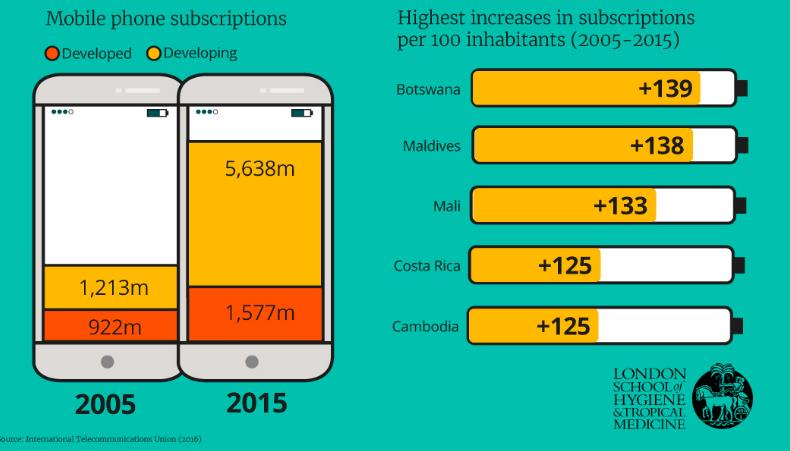
\includegraphics{Global_Mobile_Subscriptions.jpg}}
\end{figure}
\end{frame}


\begin{frame}
\frametitle{Countries with Shortage of Healthcare Providers}
\begin{figure}
\resizebox{5in}{2.5in}{\includegraphics{Shortage-Healthcare-Providers.jpg}}
\end{figure}
{\em Source: Duke Global Health Institute}
\end{frame}



\begin{frame}
\frametitle{Global Mobile Health?}
\begin{figure}
\resizebox{5in}{2.5in}{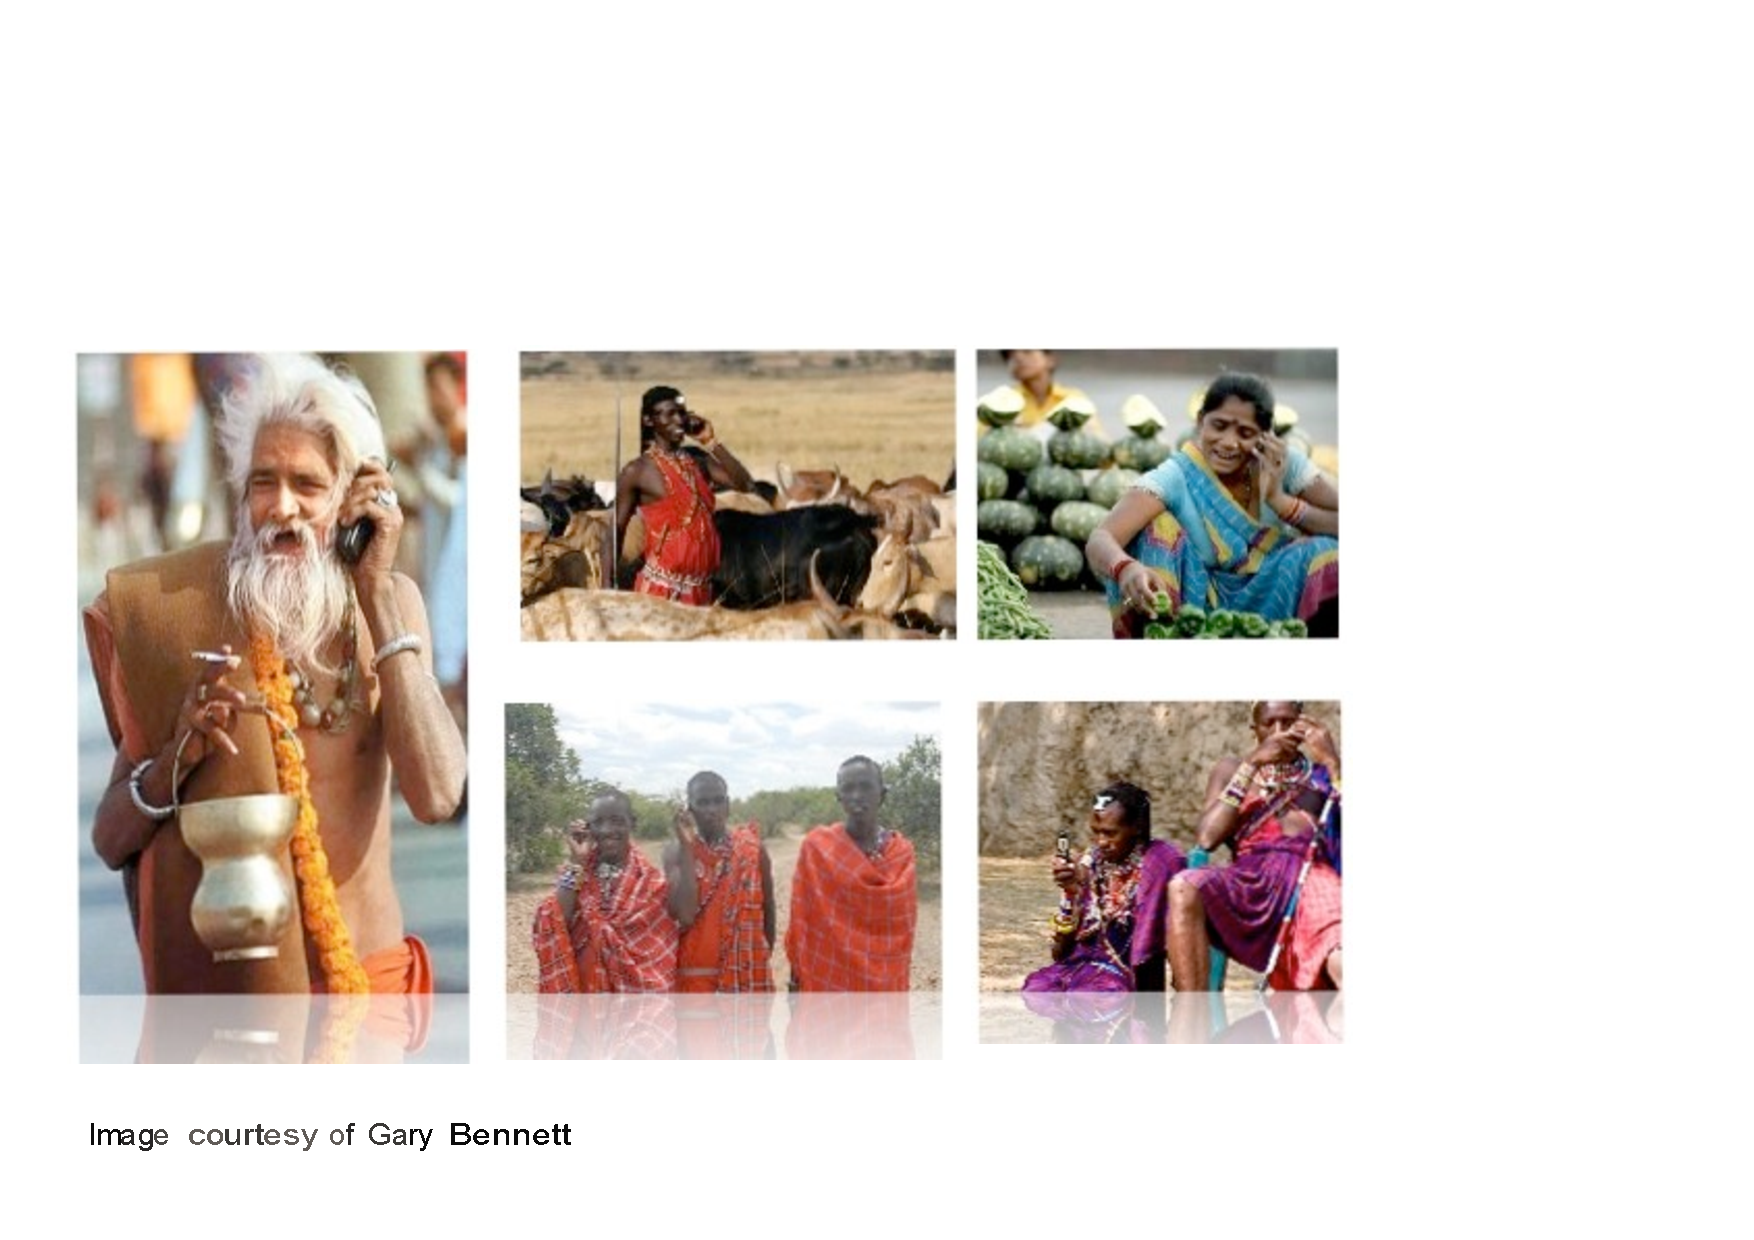
\includegraphics{Digital_Health.pdf}}
\end{figure}
{\em Source: Duke Global Health Institute}
\end{frame}




\begin{frame}
\frametitle{Acknowledgements}
\alert{Financial Support from:}
\bigskip
\begin{itemize}
\item Duke-NUS Medical School
\item Institute of Mathematical Sciences, NUS
\item Ministry of Education (MOE)
\item National Institutes of Health (NIH)
% \bigskip
% \item Intellectual support from:
% \begin{itemize}
% \item[--] Joseph Jay Williams (U-Toronto)
% \item[--] Caroline Figueroa (UC-Berkeley)
% \item[--] Susan Murphy (Harvard)
% \end{itemize}
\end{itemize}
\end{frame}




\begin{frame}[plain]
\begin{itemize}
\item Shoot your questions, comments, criticisms, request for slides to: {\color{blue}bibhas.chakraborty@duke-nus.edu.sg}\bigskip
\bigskip
\begin{center}
\begin{figure}
\resizebox{3in}{2.5in}{\includegraphics{sticky-note-thank-you-thumb.pdf}}
\end{figure}
\end{center}
\end{itemize}
\end{frame}


\end{document}








